In Exercises \ref{powereqineqexfirsta} - \ref{powereqineqexlasta}, solve the equation or inequality.  


\begin{multicols}{2}
\begin{enumerate}


\item $x+1 = (3x+7)^{\frac{1}{2}}$ \label{powereqineqexfirsta}
\item  $2x+1 = (3-3x)^{\frac{1}{2}}$

\setcounter{HW}{\value{enumi}}
\end{enumerate}
\end{multicols}

\begin{multicols}{2}
\begin{enumerate}
\setcounter{enumi}{\value{HW}}


\item  $t + (3t+10)^{0.5} = -2$
\item  $3t+(6-9t)^{0.5}=2$

\setcounter{HW}{\value{enumi}}
\end{enumerate}
\end{multicols}

\begin{multicols}{2}
\begin{enumerate}
\setcounter{enumi}{\value{HW}}

\item $x^{-1.5} = 8$
\item $2x - 1 =  (x + 1)^{-0.5}$

\setcounter{HW}{\value{enumi}}
\end{enumerate}
\end{multicols}

\begin{multicols}{2}
\begin{enumerate}
\setcounter{enumi}{\value{HW}}

\item $t^{\frac{2}{3}} = 4$
\item $(t - 2)^{\frac{1}{2}} + (t - 5)^{\frac{1}{2}} = 3$

\setcounter{HW}{\value{enumi}}
\end{enumerate}
\end{multicols}

\begin{multicols}{2}
\begin{enumerate}
\setcounter{enumi}{\value{HW}}

\item $(2x+1)^{\frac{1}{2}} = 3 + (4-x)^{\frac{1}{2}}$
\item  $5 - (4-2x)^{\frac{2}{3}} = 1$

\setcounter{HW}{\value{enumi}}
\end{enumerate}
\end{multicols}

\begin{multicols}{2}
\begin{enumerate}
\setcounter{enumi}{\value{HW}}

\item  $2t^{\frac{2}{3}} = 6 - t^{\frac{1}{3}}$  % $t=-8, \frac{27}{8}}$
\item  $2t^{\frac{1}{3}} = 1-3t^{\frac{2}{3}} $  % $t=-1, \frac{1}{27}$

\setcounter{HW}{\value{enumi}}
\end{enumerate}
\end{multicols}

\begin{multicols}{2}
\begin{enumerate}
\setcounter{enumi}{\value{HW}}

\item $2x^{1.5} = 15x^{0.75} + 8$  % $x=16$

\item  $35x^{-0.75} = x^{-1.5} +216$ % $x = \frac{1}{81}, \frac{1}{16}$

\setcounter{HW}{\value{enumi}}
\end{enumerate}
\end{multicols}

\begin{multicols}{2}
\begin{enumerate}
\setcounter{enumi}{\value{HW}}


\item  $10-\sqrt{t-2} \leq 11$ \vphantom{$t^{\frac{2}{3}} \leq 4$}
\item  $t^{\frac{2}{3}} \leq 4$ % $[-8,8]$

\setcounter{HW}{\value{enumi}}
\end{enumerate}
\end{multicols}

\begin{multicols}{2}
\begin{enumerate}
\setcounter{enumi}{\value{HW}}


\item  $\sqrt[3]{x} \leq x$   \vphantom{$(2-3x)^{\frac{1}{3}} > 3x$}
\item  $(2-3x)^{\frac{1}{3}} > 3x$  %$\left(-\infty, \frac{1}{3} \right)$

\setcounter{HW}{\value{enumi}}
\end{enumerate}
\end{multicols}

\begin{multicols}{2}
\begin{enumerate}
\setcounter{enumi}{\value{HW}}


\item  $(t^2-1)^{-\frac{1}{2}} \geq 2$  %$\left[ -\frac{\sqrt{5}}{2}, -1\right) \cup \left(1, \frac{\sqrt{5}}{2}\right]$
\item   $(t^2-1)^{-\frac{1}{3}} \leq 2$  %$\left[ -\frac{3\sqrt{2}}{4}, -1\right) \cup (-1,1) \cup \left(1, \frac{3\sqrt{2}}{4}\right]$

\setcounter{HW}{\value{enumi}}
\end{enumerate}
\end{multicols}

\begin{multicols}{2}
\begin{enumerate}
\setcounter{enumi}{\value{HW}}


\item  $3(x-1)^{\frac{1}{3}} +x (x-1)^{-\frac{2}{3}} \geq 0$ % $\left[ \frac{3}{4}, 1\right) \cup (1, \infty)$

\item $3(x-1)^{\frac{2}{3}} +2x (x-1)^{-\frac{1}{3}} \geq 0$ % $\left( -\infty, \frac{3}{5} \right] \cup (1, \infty)$

\setcounter{HW}{\value{enumi}}
\end{enumerate}
\end{multicols}


\begin{multicols}{2}
\begin{enumerate}
\setcounter{enumi}{\value{HW}}


\item  $2 (t-2)^{-\frac{1}{3}} -\frac{2}{3} t(t-2)^{-\frac{4}{3}} \leq 0$ \vphantom{$-\frac{4}{3} (t-2)^{-\frac{4}{3}} + \frac{8}{9} t (t-2)^{-\frac{7}{3}} \geq 0$}
\item  $-\frac{4}{3} (t-2)^{-\frac{4}{3}} + \frac{8}{9} t (t-2)^{-\frac{7}{3}} \geq 0$

\setcounter{HW}{\value{enumi}}
\end{enumerate}
\end{multicols}

\begin{multicols}{2}
\begin{enumerate}
\setcounter{enumi}{\value{HW}}


\item  $2x^{-\frac{1}{3}}(x-3)^{\frac{1}{3}} + x^{\frac{2}{3}} (x-3)^{-\frac{2}{3}} \geq 0$
\item $\sqrt[3]{x^{3} + 3x^{2} - 6x - 8} > x + 1$ \vphantom{ $2x^{-\frac{1}{3}}(x-3)^{\frac{1}{3}} + x^{\frac{2}{3}} (x-3)^{-\frac{2}{3}} \geq 0$}


\setcounter{HW}{\value{enumi}}
\end{enumerate}
\end{multicols}

\begin{multicols}{2}
\begin{enumerate}
\setcounter{enumi}{\value{HW}}

\item $4(7-t)^{0.75} - 3t(7-t)^{-0.25} \leq 0$  \vphantom{$4t^{0.75}(t - 3)^{-\frac{2}{3}} +9t^{-0.25}(t - 3)^{\frac{1}{3}} < 0$} %$[4, \infty)$

\item $4t^{0.75}(t - 3)^{-\frac{2}{3}} +9t^{-0.25}(t - 3)^{\frac{1}{3}} < 0$

\setcounter{HW}{\value{enumi}}
\end{enumerate}
\end{multicols}

\begin{enumerate}
\setcounter{enumi}{\value{HW}}


\item $x^{-\frac{1}{3}} (x-3)^{-\frac{2}{3}} - x^{-\frac{4}{3}} (x-3)^{-\frac{5}{3}} (x^2-3x+2) \geq 0$  \vphantom{$\frac{2}{3}(t + 4)^{\frac{3}{5}}(t - 2)^{-\frac{1}{3}} + \frac{3}{5}(t + 4)^{-\frac{2}{5}}(t - 2)^{\frac{2}{3}} \geq 0$ }
\item $\frac{2}{3}(t + 4)^{\frac{3}{5}}(t - 2)^{-\frac{1}{3}} + \frac{3}{5}(t + 4)^{-\frac{2}{5}}(t - 2)^{\frac{2}{3}} \geq 0$ \label{powereqineqexlasta}

\setcounter{HW}{\value{enumi}}
\end{enumerate}




\begin{enumerate}
\setcounter{enumi}{\value{HW}}
\item The Cobb-Douglas production model\footnote{See Example \ref{CobbDouglasEx} for more details on these sorts of models.} for the country of Sasquatchia is $P = 1.25L^{0.4}K^{0.6}$.  Here, $P$ represents the country's production (measured in thousands of Bigfoot  Bullion), $L$ represents the total labor (measured in thousands of hours) and $K$ represents the total investment in capital (measured in Bigfoot Bullion.)

\begin{enumerate}

\item \label{KintermsofLCobbexercise}Let $P = 300$ and solve for $K$ as a function of  $L$.  If $L = 100$, what is $K$?  Interpret each of the quantities in this case.

\item Graph your answer to \ref{KintermsofLCobbexercise} using a graphing utility.  What information does an ordered pair $(L, K)$ on this graph represent?  

\end{enumerate}

\end{enumerate}

\newpage

\subsection{Answers}

\begin{multicols}{3}
\begin{enumerate}


\item $x=3$  \vphantom{ $x = \frac{1}{4}$ }
\item  $x = \frac{1}{4}$
\item  $t=-3$  \vphantom{ $x = \frac{1}{4}$ }

\setcounter{HW}{\value{enumi}}
\end{enumerate}
\end{multicols}

\begin{multicols}{3}
\begin{enumerate}
\setcounter{enumi}{\value{HW}}


\item  $t = -\frac{1}{3}, \; \frac{2}{3}$  \vphantom{$x = \frac{\sqrt{3}}{2}$}
\item $x = \frac{1}{4}$  \vphantom{$x = \frac{\sqrt{3}}{2}$}
\item $x = \frac{\sqrt{3}}{2}$

\setcounter{HW}{\value{enumi}}
\end{enumerate}
\end{multicols}

\begin{multicols}{3}
\begin{enumerate}
\setcounter{enumi}{\value{HW}}


\item $t = \pm 8$
\item $t = 6$
\item  $x = 4$

\setcounter{HW}{\value{enumi}}
\end{enumerate}
\end{multicols}

\begin{multicols}{3}
\begin{enumerate}
\setcounter{enumi}{\value{HW}}
 
\item  $x=-2, 6$  \vphantom{$t=-8, \frac{27}{8}$}
\item   $t=-8, \frac{27}{8}$
\item   $t=-1, \frac{1}{27}$   \vphantom{$t=-8, \frac{27}{8}$}

\setcounter{HW}{\value{enumi}}
\end{enumerate}
\end{multicols}

\begin{multicols}{3}
\begin{enumerate}
\setcounter{enumi}{\value{HW}}

\item $x=16$ \vphantom{$x = \frac{1}{81}, \frac{1}{16}$}
\item  $x = \frac{1}{81}, \frac{1}{16}$
\item  $[2, \infty)$   \vphantom{$x = \frac{1}{81}, \frac{1}{16}$}


\setcounter{HW}{\value{enumi}}
\end{enumerate}
\end{multicols}

\begin{multicols}{3}
\begin{enumerate}
\setcounter{enumi}{\value{HW}}

\item  $[-8,8]$    \vphantom{ $\left(-\infty, \frac{1}{3} \right)$}
\item  $[-1, 0] \cup [1, \infty)$  \vphantom{ $\left(-\infty, \frac{1}{3} \right)$}
\item $\left(-\infty, \frac{1}{3} \right)$

\setcounter{HW}{\value{enumi}}
\end{enumerate}
\end{multicols}

\begin{multicols}{2}
\begin{enumerate}
\setcounter{enumi}{\value{HW}}

\item $\left[ -\frac{\sqrt{5}}{2}, -1\right) \cup \left(1, \frac{\sqrt{5}}{2}\right]$
\item  $\left(-\infty, -\frac{3\sqrt{2}}{4} \right] \cup (-1,1) \cup \left[ \frac{3\sqrt{2}}{4}, \infty \right)$

\setcounter{HW}{\value{enumi}}
\end{enumerate}
\end{multicols}

\begin{multicols}{2}
\begin{enumerate}
\setcounter{enumi}{\value{HW}}


\item   $\left[ \frac{3}{4}, 1\right) \cup (1, \infty)$

\item $\left( -\infty, \frac{3}{5} \right] \cup (1, \infty)$

\setcounter{HW}{\value{enumi}}
\end{enumerate}
\end{multicols}

\begin{multicols}{2}
\begin{enumerate}
\setcounter{enumi}{\value{HW}}

\item  $(-\infty, 2) \cup (2,3]$
\item  $(2,6]$

\setcounter{HW}{\value{enumi}}
\end{enumerate}
\end{multicols}

\begin{multicols}{2}
\begin{enumerate}
\setcounter{enumi}{\value{HW}}

\item $(-\infty, 0) \cup [2,3) \cup (3, \infty)$
\item $(-\infty, -1)$  


\setcounter{HW}{\value{enumi}}
\end{enumerate}
\end{multicols}

\begin{multicols}{2}
\begin{enumerate}
\setcounter{enumi}{\value{HW}}

\item $[4,7)$  \vphantom{$\left(0, \frac{27}{13} \right)$}
\item $\left(0, \frac{27}{13} \right)$

\setcounter{HW}{\value{enumi}}
\end{enumerate}
\end{multicols}

\begin{multicols}{2}
\begin{enumerate}
\setcounter{enumi}{\value{HW}}
\item $(-\infty, 0) \cup (0,3)$   \vphantom{$(-\infty, -4) \cup \left(-4, -\frac{22}{19}\right] \cup (2, \infty)$}
\item $(-\infty, -4) \cup \left(-4, -\frac{22}{19}\right] \cup (2, \infty)$

\setcounter{HW}{\value{enumi}}
\end{enumerate}
\end{multicols}

\begin{enumerate}
\setcounter{enumi}{\value{HW}}
\item \begin{enumerate}

\item $K=f(L) = (240)^{ \frac{5}{3}} L^{- \frac{2}{3}}$.  $f(100)  \approx 430.2148$.  This means in order for the production level of Sasquatchia to reach 300,000 Bigfoot Bullion with a labor investment of 100,000 hours, the country needs to invest approximately 430 Bigfoot Bullion into capital.


\item If a point $(L,K)$ is on the graph of this function, it means a combination of $L$ thousand hours of labor with an investment of $K$ Bigfoot Bullion into the Sasquatian Economy will result in a production level of 300,000 Bigfoot Bullion.

\centerline{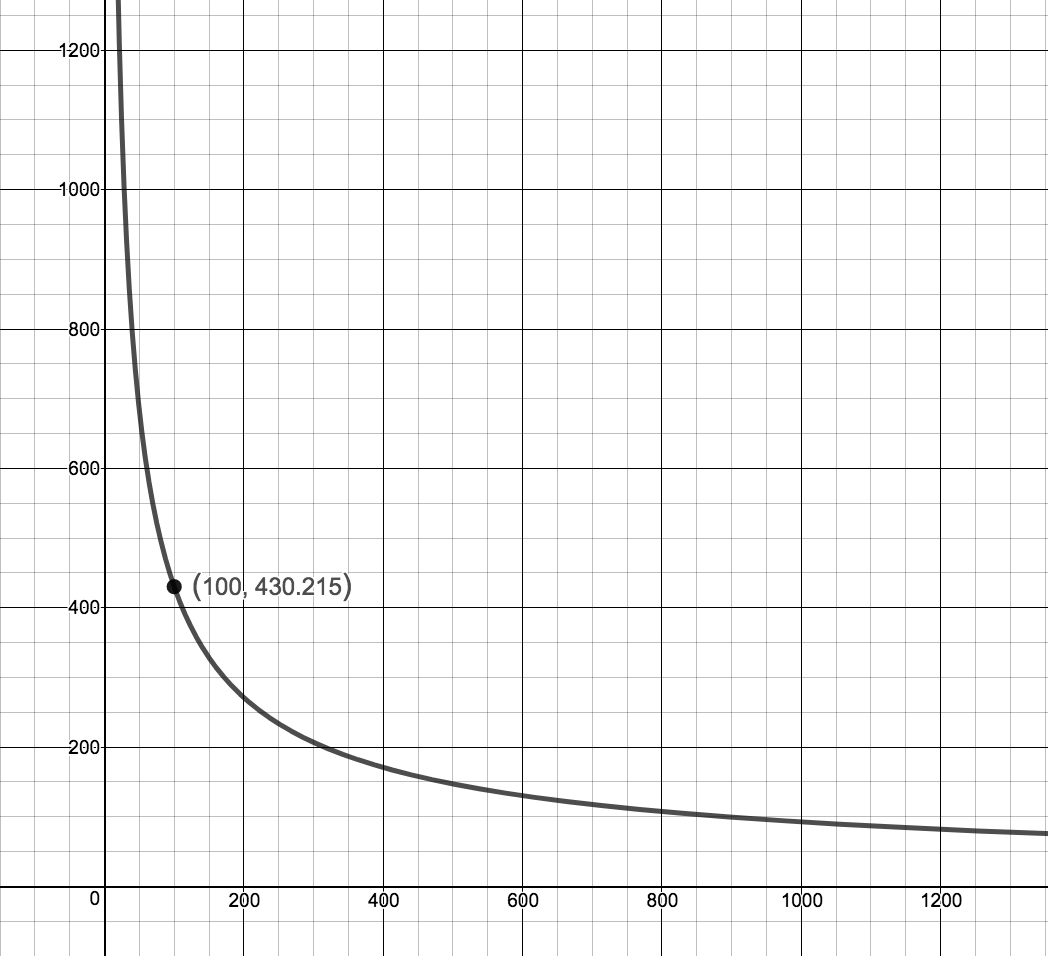
\includegraphics[height=2in]{./PowerEqIneqGraphics/CobbDouglasExercise.jpg}}



\end{enumerate}

\end{enumerate}